\documentclass[12pt, ngerman]{article}

% Zitieren
%\usepackage{biblatex-chicago}
\usepackage[backend=biber]{biblatex-chicago}
\addbibresource{main2.bib}
\usepackage{biblatex}
\interfootnotelinepenalty=10000
% Packages
%test

\usepackage[ngerman]{babel}
\usepackage{csquotes}
\MakeOuterQuote{"}

%\usepackage{color}
%\usepackage{amssymb}
\usepackage{amsthm}
\usepackage{graphicx}
\usepackage{pgf-pie}
\usepackage{pgfplots}
%\usepackage[section]{placeins}
\graphicspath{{images/}}

\usepackage[a4paper,margin=3cm]{geometry}
\usepackage[onehalfspacing]{setspace}

\usepackage[pdftex,pdfpagelabels,bookmarks,hyperindex,hyperfigures]{hyperref}
\usepackage{tikz}
\usepackage{siunitx}
\usepackage{booktabs}
\usepackage{amsmath}
\usepackage[nameinlink]{cleveref}
\usepackage[utf8]{inputenc}
\usepackage[T1]{fontenc}




\sisetup{locale = DE}

\newcommand{\pe}{_{\text{PE}}}
\newcommand{\el}{_{\text{el}}}

% Document
\begin{document}

    \begin{titlepage}


        \title{Bidirektionales Laden}
        \author{David Behres}
        \date{2022}
        \maketitle

    \end{titlepage}

    \tableofcontents
    \pagebreak


    \section{Bewältigung der Klima- und Energiekrise und die Rolle von E-Autos}



    Sowohl der Klimawandel als auch der internationale Konflikt zwischen der Ukraine und Russland zeigen die Probleme
    der deutschen Stromversorgung auf.
    Deutschlands Energieerzeugung erfolgt zu 52,1\% aus konventionellen oder fossilen Energiequellen, die der Umwelt
    schaden.
    Die Abhängigkeit von konventionellen Energien treten in der Regel wegen Mangel an erneuerbaren Energien auf.
    Weitere Probleme sind der Import von Strom bei Produktionsmangel und Export von Strom bei Produktionsüberschuss.
%Zudem reicht die interne Energieproduktion manchmal, besonders bei windstillen Nächten, nicht aus, um den
%Energieverbrauch abzudecken, wodurch Strom importiert werden muss.
%Umgekehrt kommt es bei hoher Sonnen- und Windstärke oft zu Energieüberschuss.
%Da es nicht genügend Kapazitäten gibt, um diese überschüssige Energie zu speichern, muss sie exportiert werden.

    \subsection{Abhängigkeit von russischem Gas und Öl} \label{subsec:putin}
    Russland führt derzeit einen grausamen und unnötigen Überfall auf die Ukraine aus.
    Um Russland zu schwächen haben viele Staaten Sanktionen verhängt, welche das Land unter anderem Wirtschaftlich
    schwächen sollen.\footcite{SanktionenGegenRussland2022}
    Dennoch bezieht Deutschland weiterhin hohe Mengen and Öl und Erdgas aus Russland, da es von diesen und
    unterstützt damit indirekt den Krieg.


    Im vergangenen Jahr bezog Deutschland 55\% des Erdgas aus Russland, gegen Ende dieses Jahres will man dies auf
    30\% verringern.\footcite{wdraktuellFAQWasGasLieferstopp} Dennoch wird das nicht reichen um Russland merkbar zu
    Schwächen, denn durch die vom Krieg verursachten hohen Gaspreise wird Deutschland nach Schätzungen der
    Umweltorganisation Greenpeace Rekordsummen an Russland für Erdgas und Öl und zahlen und dadurch den russischen
    Krieg finanzieren.\footcite{balserOlUndGas}

    \subsection{Abhängigkeit von fossilen Brennstoffen und deren Einfluss auf den Klimawandel}

    Der Anteil an konventionellen Energieträgern an der Stromerzeugung lag im 1.\ Quartal 2022 bei 52,1\%.
    Die Verwendung solcher fossiler Brennstoffe, wie Braunkohle oder Erdgas, hat durch die Erzeugung von
    Treibhausgasen einen schädlichen Einfluss auf den Klimawandel.\footcite{wilkeErneuerbareUndKonventionelle2013}

    \subsection{Energieträger und ihre Umweltauswirkungen}

    \subsubsection{Statistiken und Erklärungen zur aktuellen Lage in Deutschland}\label{subsec:primar}

    Der Energieverbrauch in Deutschland wird durch unterschiedliche Energieträger gedeckt.
    Diese Energieträger unterscheiden sich unter anderem in ihrem Umwelteinfluss.

    Das folgende Diagramm unterteilt den Primärenergieverbrauch des Jahres 2020 von
    \qty{11.895}{PJ\pe}\footnote{PE steht für Primärenergie}
    in die unterschiedlichen Energieträger.
    Der Primärenergieverbrauch bezeichnet den Energiegehalt der verwendeten Energieträger und hängt unter anderem vom
    Wirkungsgrad ab.

    \begin{figure}[!h]
        \begin{tikzpicture}
            \pie[text=legend, sum=auto, radius=2, color={blue, yellow, gray, brown, lightgray, green, teal}]{
                4087/Öl,
                3144/Gas,
                896/Steinkohle,
                958/Braunkohle,
                702/Kernenergien,
                1972/Erneuerbare Energien,
                136/Sonstige Energieträger}
        \end{tikzpicture}\caption{Primärenergieverbrauch nach Energieträger 2020 in \unit{PJ\pe}}
        \label{fig:pie}
    \end{figure}

    Davon wurden etwa \qty{1482}{PJ\pe} Erdgas zum Heizen verwendet, sowie \qty{576}{PJ\pe}
    zur Erzeugung von Prozesswärme in der Industrie, \qty{384}{} und \qty{177}{PJ\pe} für Eigenstromerzeugung in der
    Industrie verwendet.\footcite{Industrie, Energieflussbild2020PJLang, WieKannTransformation}

    Der Mineralölverbrauch für das Heizen beträgt \qty{809}{PJ\pe}, für Fahrzeuge \qty{1642}{PJ\pe}
    und für Flugzeuge \qty{335}{PJ\pe}.\footcite{Energieflussbild2020PJLang,
        wilkeEndenergieverbrauchUndEnergieeffizienz2013}

    \subsubsection{Elektrische Energie}

    Von der Stromerzeugung des Jahres 2021 von \qty{1819}{PJ\el} wurden \qty{353}{PJ\el} mit Braunkohle,
    \qty{139}{PJ\el} mit Gas und \qty{187}{PJ\el} Steinkohle mit produziert.\footcite{SMARDEntwicklungenIm}.
    Allerdings ist es wichtig diese Menge nicht mit den anderen zu vergleichen, da es sich um die Erzeugnisse in
    elektrischer Energie handelt.

    Energien müssen je nach Nutzen in eine bestimmte Energieform gebracht werden.
    Dazu werden die an die Energieträger gebundenen Energien mit chemischen und technischen Prozessen in die
    gewünschte Form gebracht.
    Beispielsweise kann die an Brennstoffen gebundene chemische Energie in thermische umgewandelt werden, wobei
    Treibhausgase freigesetzt werden.
    Diese kann anschließend zum Heizen oder in der Industrie verwendet werden aber auch in Kraftwerken weiter zu
    elektrischer Energie verarbeitet werden.
    Dabei kommt allerdings, je nach Wirkungsgrad des Kraftwerks,
    ein großer Teil der Energie als Wärmeenergie abhanden.\footcite{AachenHatEnergie}

    Um später die Emissionen zu berechnen, müssen die elektrischen Energiemengen zuerst in Primärenergie umgewandelt
    werden

    Der Wirkungsgrad \unit{\eta} ist allgemein definiert als
    \(\eta=\frac{E_{\text{nutz}}}{E_{\text{ges}}}\).\footcite{WirkungsgradLEIFIphysik}
    Hier entspricht \(E_\text{nutz}\) \(E\el\) und \(E_\text{{ges}}\) \(E\pe\).
    Durch Umformen ergibt sich: \[E\pe=\frac{E\el}{\eta}\]



    Aus den durchschnittlichen Wirkungsgraden der Kraftwerke lässt sich die elektrische Energieproduktion des Jahres
    2021 in \qty{385}{PJ\pe} Gas,
    \qty{896}{PJ\pe} Braunkohle und \qty{429}{PJ\pe} Steinkohle umrechnen
    .\footcite{wilkeKraftwerkeKonventionelleUnd2013}

    Der niedrige zeitliche Abstand der hier verwendeten Daten (2021) zu den in \cref{subsec:primar} (2020)
    wird in den nächsten Abschnitten ignoriert.

    \subsubsection{Zusammenfassung des Energieverbrauchs und dessen Emissionen}

    Die Emissionen von Treibhausgasen, die durch die Förderung und den Verbrauch von konventionellen Energieträgern
    entstehen, sind eine der größten Antreiber des Klimawandels.
    Die Menge der Emissionen variiert je nach Energieträger.
    Die folgende Tabelle listet diese sogenannten "Emissionsfaktoren" in \unit{tCO^2/PJ\pe} auf
    .\footcite{balserOlUndGas}
%direkte emissionsfaktoren

    \begin{center}
        \begin{tabular}{r|l}
            \toprule
            Energieträger & Emissionsfaktor \\
            \midrule
            Erdgas        & 55              \\
            Mineralöl     &  75              \\
            Steinkohle    & 101             \\
            Braunkohle    & 98              \\
            \bottomrule
        \end{tabular}
    \end{center}

    \paragraph{Zusammenfassung}

    Die folgende Grafik ist eine Zusammenfassung der bisher ermittelten Energieverbräuche und ihrer Anwendungen in
    \unit{PJ\pe}.

    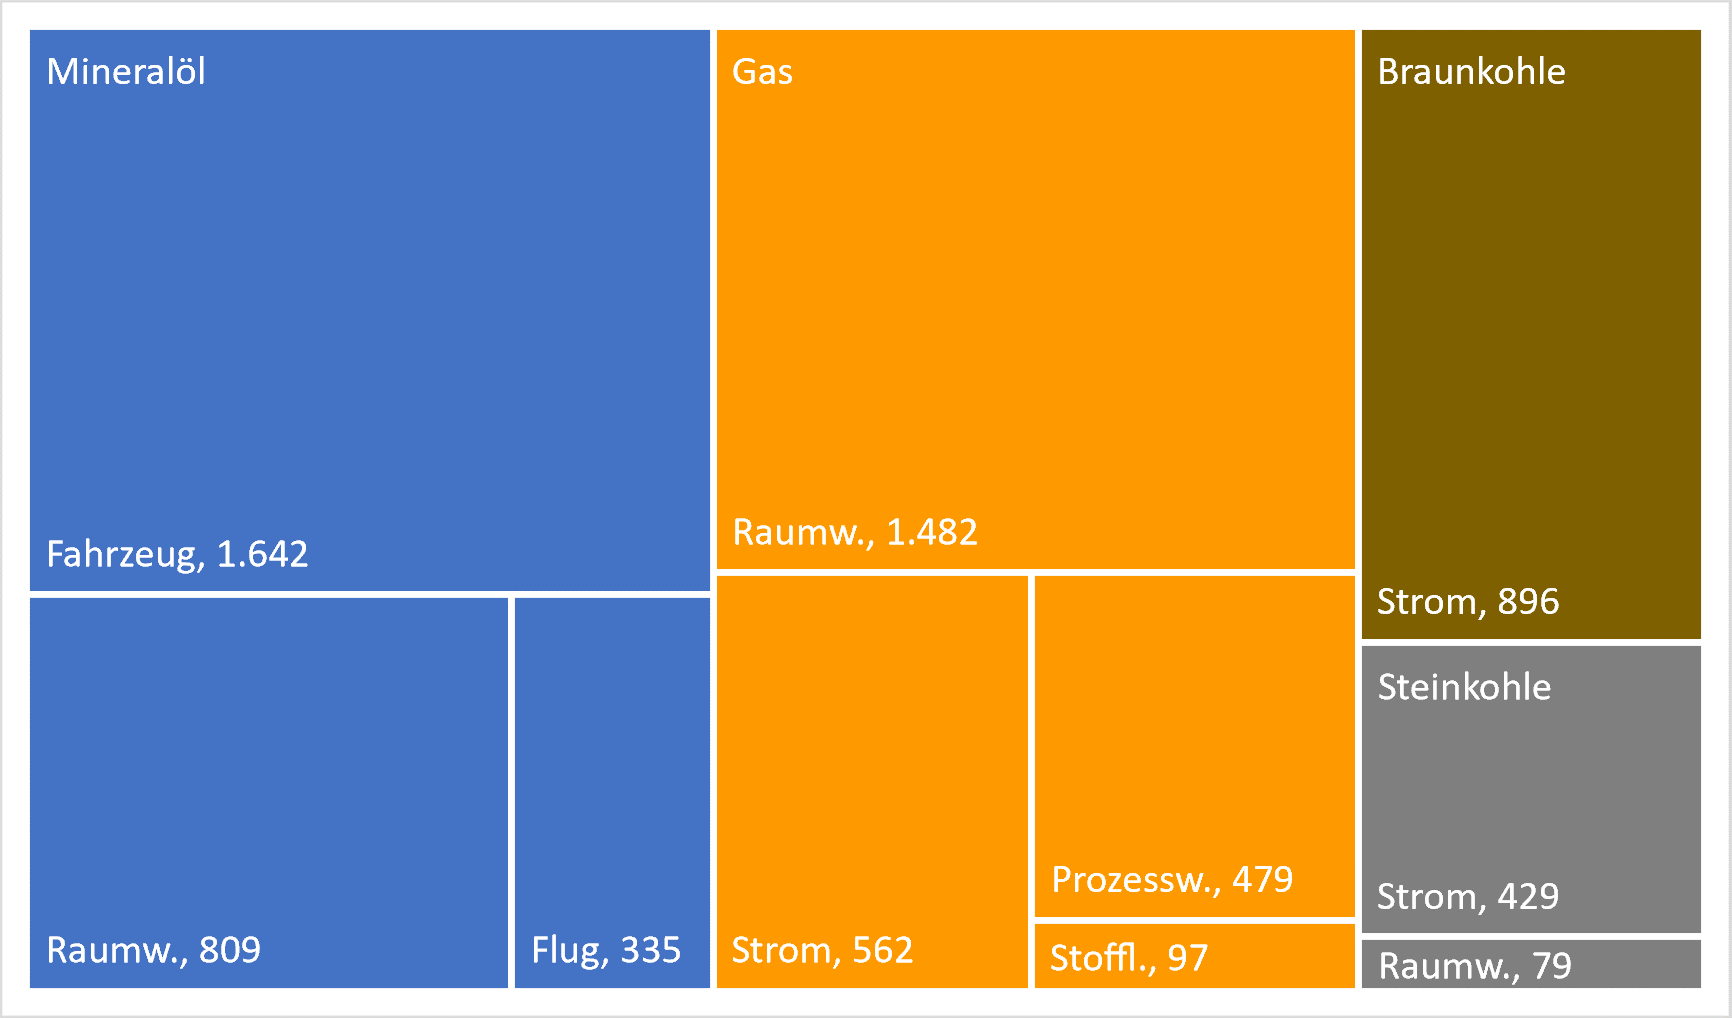
\includegraphics{anwendung}

    Die Summe dieser Energien beträgt \qty{6809}{PJ\pe}, was über der Hälfte des Primärenergieverbrauchs liegt und
    somit auch in etwa die Hälfte der Emissionen erzeugt.
    In den folgenden Abschnitten wird sich damit befasst werden, wie man diese durch Alternativen vermeiden kann und
    welche rolle das bidirektionale Laden spielen könnte.

    Als Alternative zum Heizen mit fossilen Brennstoffen bietet sich das Heizen mit Wärmepumpen an, welche etwa
    \unit{\frac{2}{3}} der Energie aus der Umgebung entziehen.

    Als Alternative zum Verbrauch von fossilen Kraftstoffen im Verkehr bietet sich das Fahren von Elektroautos an.
    Der Kraftstoffverbrauch macht einen großen Teil des Gesamtenergieverbrauchs aus, und wirkt sich damit sehr
    negativ auf den Klimawandel aus.

    Damit beide oben genannten Lösungsansätze umgesetzt werden können, müssen höhere Stromkapazitäten vorhanden sein.
    Diese müssten außerdem durch erneuerbare Energien abgedeckt werden.
    Auch die bereits von konventionellen Energieträgern abgedeckten Stromkapazitäten werden durch regenerative
    Abgedeckt werden müssen.

    \subsection{Lösungsansätze und Maßnahmen zur Vermeidung von Emissionen}

    Dieser Abschnitt wird verschiedene Lösungsansätze Erklären und Bewerten.
    Eine der wichtigsten Kriterien hierbei ist die Effizienz der Umweltschonung zum Energieverbrauch, also das
    Verhältnis von eingesparten Treibhausgasen zur verbrauchten Energie.
    Dieses "Einsparungseffizienz" $S$ lässt sich in
    \(\frac{\si{m}}{\si{E\el}}\) angeben, also der eingesparten Masse an \si{CO_{2}} Gasen pro verbrauchter Energie.
    Je höher dieser Wert, umso besser.
    Die folgenden Lösungsansätze werden zeigen, wie regenerative, elektrische Energie alternativ statt fossile
    Energieträger verwendet werden könnte.

    \subsubsection{Künstliche Herstellung von Energieträgern}
    Derzeit werden Energieträger wie Gas - also Methan - und Öl fast ausschließlich auf umweltbelastende Art fossil
    gefördert.
    Stattdessen könnten diese chemisch durch Strom hergestellt werden.

    \paragraph{Mineralöl}


    Künstliches Mineralöl, auch als E-Fuels bezeichnet, werden durch synthese von Wasserstoff und Kohlenstoff
    hergestellt.
    Der Wasserstoff wird dabei durch Elektrolyse gewonnen und der Kohlenstoff aus der Umgebung
    gesammelt\footcite{EFuel2022}.
    Der Wirkungsgrad dieser Umwandlung beträgt derzeit nur etwa 40\%, können allerdings laut aktuellen Forschungen
    auf bus zu 60\% steigen.
    Da diese Branche noch relativ neu ist, wird hier in die Zukunft blickend mit einem großzügigen Wirkungsgrad von
    55\% gearbeitet

    Die Einsparungseffizienz \(S_{\text{efuel}}\) wird aus dem Produkt des Emissionsfaktor \(F_{\text{öl}}\) von
    \(75\frac{t}{PJ_{\text{öl}}}\)
    und dem Gesamtwirkungsgrad \(\eta_{\text{efuels}}\) dieser Lösung von $0,55\frac{PJ_{\text{öl}}}{PJ\el}$ berechnet.


    \[S_\text{efuel} = F_{\text{öl}} \cdot \eta_{\text{efuels}} = 75\frac{t}{\text{PJ}_{\text{öl}}} \cdot 0,
    55\frac{PJ_\text{öl}}{PJ\el} = 41,25\frac{}{}\] 

    \subsection{Mangelnde Kapazitäten des Stromnetz um Heizträger zu ersetzen}

    Bei direkter Betrachtung des Anteils von Erdgas bei der Stromerzeugung von etwa 10\% scheint Erdgas zunächst kein
    großer Faktor in der elektrischen Stromversorgung zu sein.\footcite{SMARDHoherEEAnteil,EnergieWofurErdgas}
    Betrachtet man jedoch, dass Erdgas über die Hälfte des in Deutschland verbrauchten Energie ausmacht und
    hauptsächlich zum Heizen verwendet wird\footcite{Anwendungsbereiche,EnergieWofurErdgas},
    während nur zu 5,6\% mit elektrischer Energie geheizt wird, erkennt man schnell, dass Deutschland sehr von diesen
    fossilen Brennstoffen (aus Russland) abhängig ist.
    Dies liegt daran, dass das Deutsche Stromnetz nicht die nötigen Kapazitäten hat, um diese zu ersetzen
    .\footcite{EnergieWofurErdgas}

    \subsection{Unzuverlässigkeit der Erneuerbaren}
    Dass die erweiterte Nutzung der erneuerbaren Energien unabdingbar für die Lösung des deutschen Energieproblemes
    ist, sollte nun belegt sein.
    Allerdings sind die darunter relevanten Energiequellen, Wind und Sonne, nicht zuverlässig, da sie von
    variierenden Umweltfaktoren abhängen.
    Zu schlechten Zeiten würde selbst bei einem Ausbau von diesen die Stromversorgung auf konventionelle Energien und
    Importe zurückfallen.
    Um das zu vermeiden braucht es hohe Speicherkapazitäten.

    \subsection{Produktionsüberschuss bei Fotovoltaik-Ausbau}
    Bei Nutzung der verfügbaren Fläche für Fotovoltaikanlagen würde es bei dem derzeitigen Stromnetz, Verbrauch und
    Speicherkapazitäten ohne Zweifel zu einem Produktionsüberschuss kommen.\footcite{wirthAktuelleFaktenZur}
    Der Ausbau wäre also bis zu einem bestimmten Punkt nicht mehr sinnvoll, da es an Speicherkapazitäten fehlt.
    Dieses Problem könnte durch Bidirektionales Laden gelöst werden.


    \section{Bidirektionales Laden als Lösung}

    \subsection{Vehicle to Home}

    \subsection{Vehicle to Grid \& Einspeisung}

    \subsection{Auswirkungen auf Batterielebensdauer}

    \subsection{Aktueller Fortschritt}


    \section{Experiment: 12V Batterie}

    \subsection{Versuchsaufbau}

\end{document}

